\documentclass{article}
\usepackage{graphicx}
\usepackage{caption}
\usepackage{amsmath} % For math symbols and commands
\usepackage{amssymb} % For additional symbols
\usepackage{graphicx} % For graphics
\usepackage{hyperref} % For hyperlinks (optional)
\usepackage{xspace} % For spacing after LaTeX commands
\usepackage{ragged2e}
\usepackage{listings}
\usepackage{xcolor}

\definecolor{codegray}{rgb}{0.5,0.5,0.5}
\definecolor{codeblue}{rgb}{0.1,0.1,0.8}
\definecolor{codegreen}{rgb}{0,0.6,0}
\definecolor{backcolour}{rgb}{0.996,0.976,0.949}

% Configure the listing style
\lstdefinestyle{mystyle}{
    commentstyle=\color{codegreen},
    keywordstyle=\color{codeblue},
    numberstyle=\tiny\color{codegray},
    stringstyle=\color{codegreen},
    basicstyle=\ttfamily\footnotesize,
    breakatwhitespace=false,
    breaklines=true,
    captionpos=b,
    keepspaces=true,
    numbersep=5pt,
    showspaces=false,
    showstringspaces=false,
    showtabs=false,
    tabsize=2
}
\lstset{style=mystyle}



\begin{document}

\vspace{4cm} 

\begin{center}
    \begin{minipage}{0.45\textwidth}
        \centering
        \includegraphics[width=\textwidth]{/Users/mac/Desktop/MST AISD/Documents/fstt.png}
    \end{minipage}
    \hspace{0.05\textwidth}
    \begin{minipage}{0.45\textwidth}
        \centering
        \includegraphics[width=\textwidth]{/Users/mac/Desktop/MST AISD/Documents/univ.png}
    \end{minipage}
\end{center}
\vspace{5cm}
\noindent\rule{\linewidth}{1.5pt}
\begin{center}
    \textbf{\LARGE CNN Assignment Report   }
\end{center}
\noindent\rule{\linewidth}{1.5pt}
\vspace{2cm}
\begin{center}
\textbf{Authors:} \hspace{1cm} \\
\vspace{0.5cm}
\textbf{Abdelmajid Benjelloun} \\
\vspace{0.2cm}
\textit{20000203}\\
\vspace{0.2cm}

\textit{H130407540}\\
\vspace{0.2cm}


\textbf{Supervisor:} \\
\vspace{0.5cm}
\textbf{Pr. ...... ......}\\
\date{October 2024}
\end{center}

\newpage
\tableofcontents

\newpage

\section{Questions for Custom CNN}
\subsection{What are the steps for data preprocessing to build a custom CNN?}

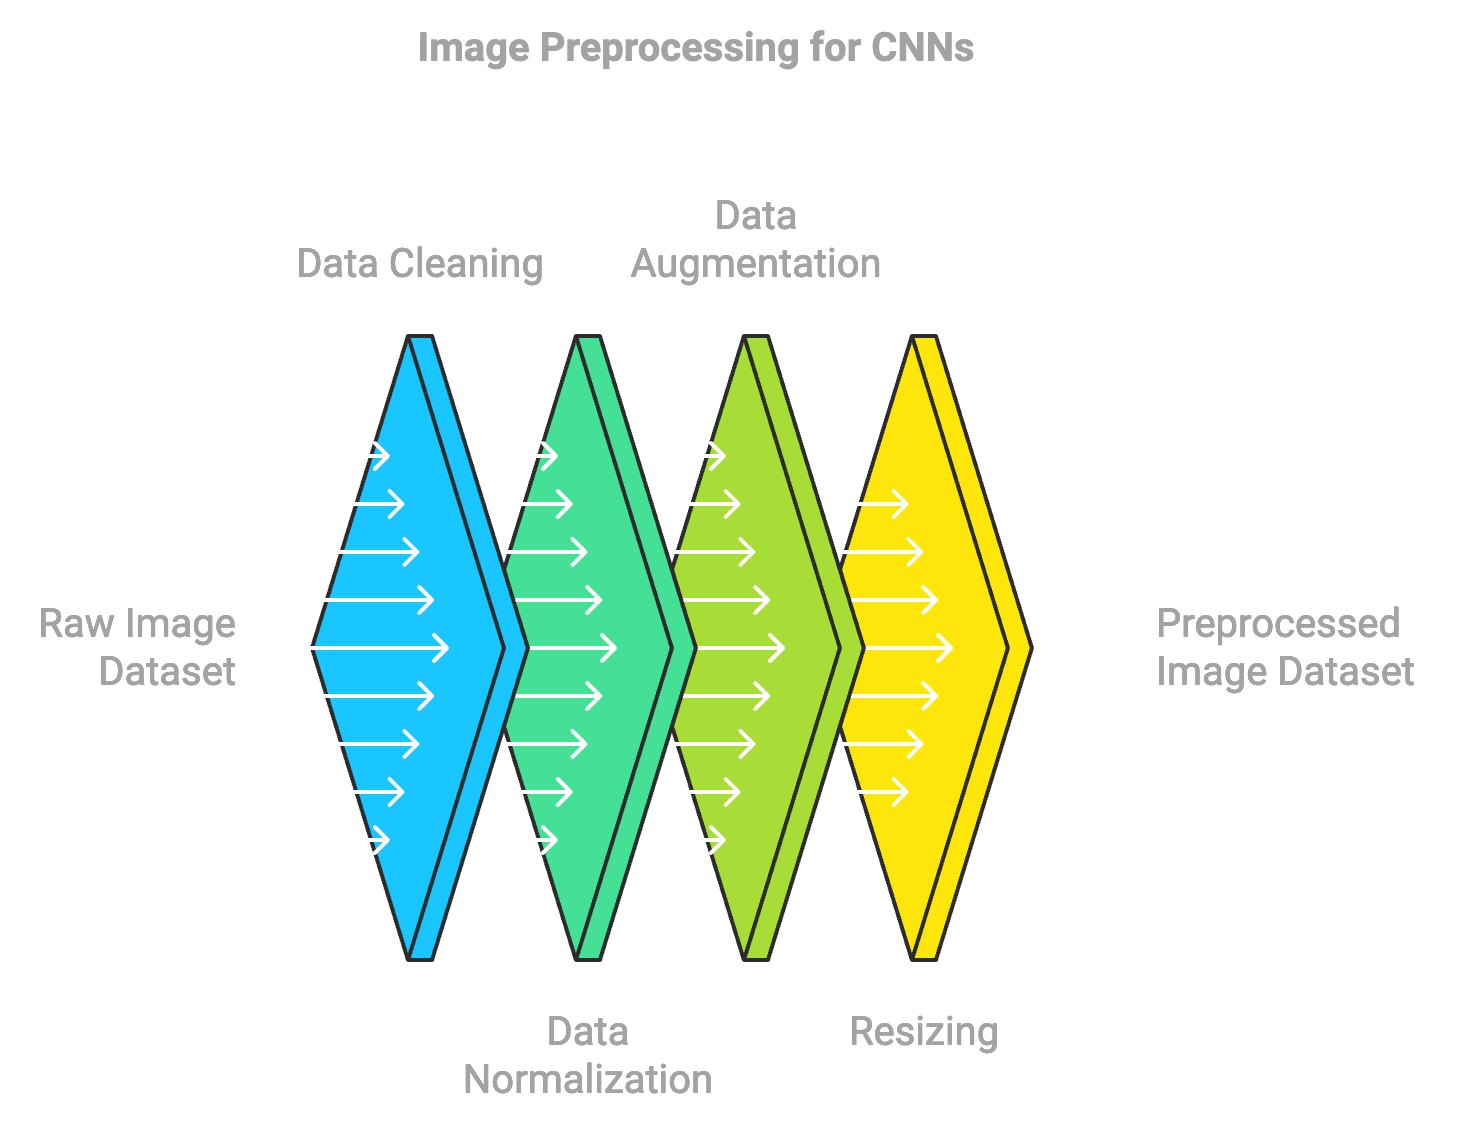
\includegraphics[width=\textwidth,height=0.35\textheight,keepaspectratio]{/Users/mac/Desktop/MST AISD/S3/Transfert Learning/TP/Image/napkin-selection (2).png}


Data preprocessing is crucial in building a Convolutional Neural Network (CNN) to ensure the data is clean, normalized, and ready for efficient training. The main steps for data preprocessing include:

\begin{itemize}
    \item \textbf{Data Cleaning:} Removing or handling missing, incomplete, or corrupted data to maintain consistency.
    \item \textbf{Data Normalization:} Scaling pixel values, usually to a range between 0 and 1 or -1 and 1. This can be mathematically represented as:
    \[
    x_{\text{normalized}} = \frac{x - \text{min}(x)}{\text{max}(x) - \text{min}(x)}
    \]
    where \( x \) represents the original pixel value, and \(\text{min}(x)\) and \(\text{max}(x)\) are the minimum and maximum pixel values, respectively.
    \item \textbf{Data Augmentation:} Applying transformations, such as rotation, flipping, and scaling, to artificially increase dataset diversity. For example, a rotation transformation on an image \( I \) by angle \( \theta \) can be represented as:
    \[
    I' = R(\theta) \cdot I
    \]
    where \( R(\theta) \) is the rotation matrix.
    \item \textbf{Resizing:} Ensuring that all images are resized to a consistent input size, such as \(224 \times 224\) or \(32 \times 32\), to maintain uniform input dimensions for the CNN.
\end{itemize}

\subsection{How do we build the different layers of a custom CNN?}

Constructing a custom CNN involves defining several types of layers, each responsible for specific operations:

\begin{itemize}
    \item \textbf{Convolutional Layers:} These layers apply a set of filters (kernels) to the input data. The convolution operation between an input \( X \) and a kernel \( K \) can be represented as:
    \[
    (X * K)(i, j) = \sum_m \sum_n X(i+m, j+n) \cdot K(m, n)
    \]
    where \( (i, j) \) denotes the position in the output feature map.
    \item \textbf{Activation Layers:} Non-linear activation functions like ReLU (Rectified Linear Unit) are applied. ReLU is defined as:
    \[
    f(x) = \max(0, x)
    \]
    This introduces non-linearity, enabling the model to learn complex patterns.
    \item \textbf{Pooling Layers:} Max-pooling or average-pooling layers downsample the feature maps. For max-pooling with a \(2 \times 2\) filter, the output at each position is:
    \[
    \text{max-pool}(i, j) = \max(X_{i:i+2, j:j+2})
    \]
    \item \textbf{Fully Connected Layers:} These layers connect every neuron in the previous layer to each neuron in the current layer, enabling the model to make final predictions.
    \item \textbf{Dropout Layers:} These layers randomly drop a fraction \(p\) of neurons during training to reduce overfitting. If \( p = 0.5 \), then approximately half of the neurons are randomly dropped.
\end{itemize}
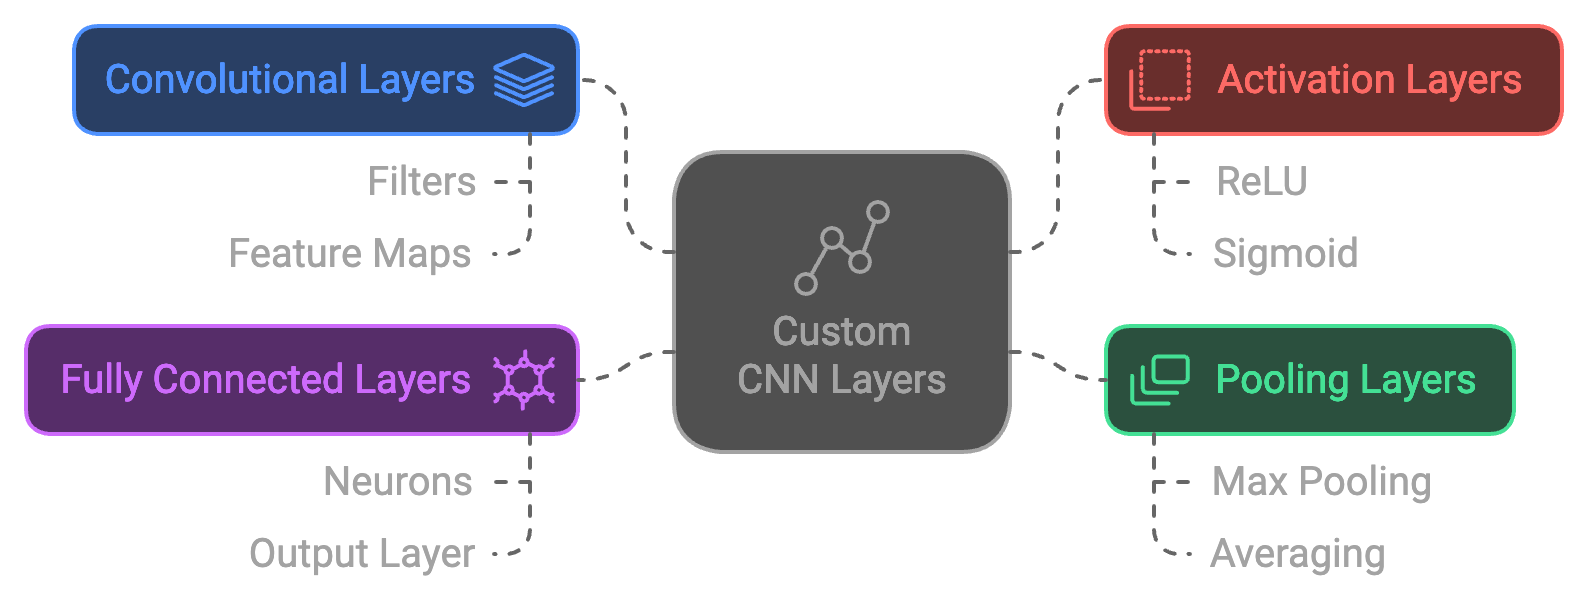
\includegraphics[width=\textwidth,height=0.25\textheight,keepaspectratio]{/Users/mac/Desktop/MST AISD/S3/Transfert Learning/TP/Image/napkin-selection (1).png}

\subsection{Which hyperparameters are critical in a custom CNN?}

Critical hyperparameters in a custom CNN directly influence the model’s performance and include:

\begin{itemize}
    \item \textbf{Learning Rate:} Controls the step size for updating weights during training. A typical gradient update can be expressed as:
    \[
    w_{t+1} = w_t - \alpha \cdot \nabla L(w_t)
    \]
    where \( w \) represents the weights, \( \alpha \) is the learning rate, and \( \nabla L(w_t) \) is the gradient of the loss \( L \).
    \item \textbf{Batch Size:} Determines the number of samples processed before updating weights. Larger batch sizes allow for more stable gradient estimates, but smaller batches allow faster updates.
    \item \textbf{Number of Filters:} The number of filters in each convolutional layer impacts the model’s capacity to learn features, as each filter captures a unique aspect of the input.
    \item \textbf{Kernel Size:} The size of the filters used in convolutional layers, often represented as \(3 \times 3\) or \(5 \times 5\). A kernel size of \(3 \times 3\) is common due to its efficiency in capturing spatial patterns.
    \item \textbf{Number of Epochs:} Defines the total number of complete passes through the training data.
    \item \textbf{Dropout Rate:} Controls the proportion of neurons randomly dropped in dropout layers. For example, a dropout rate \( p = 0.5 \) will drop half of the neurons.
\end{itemize}
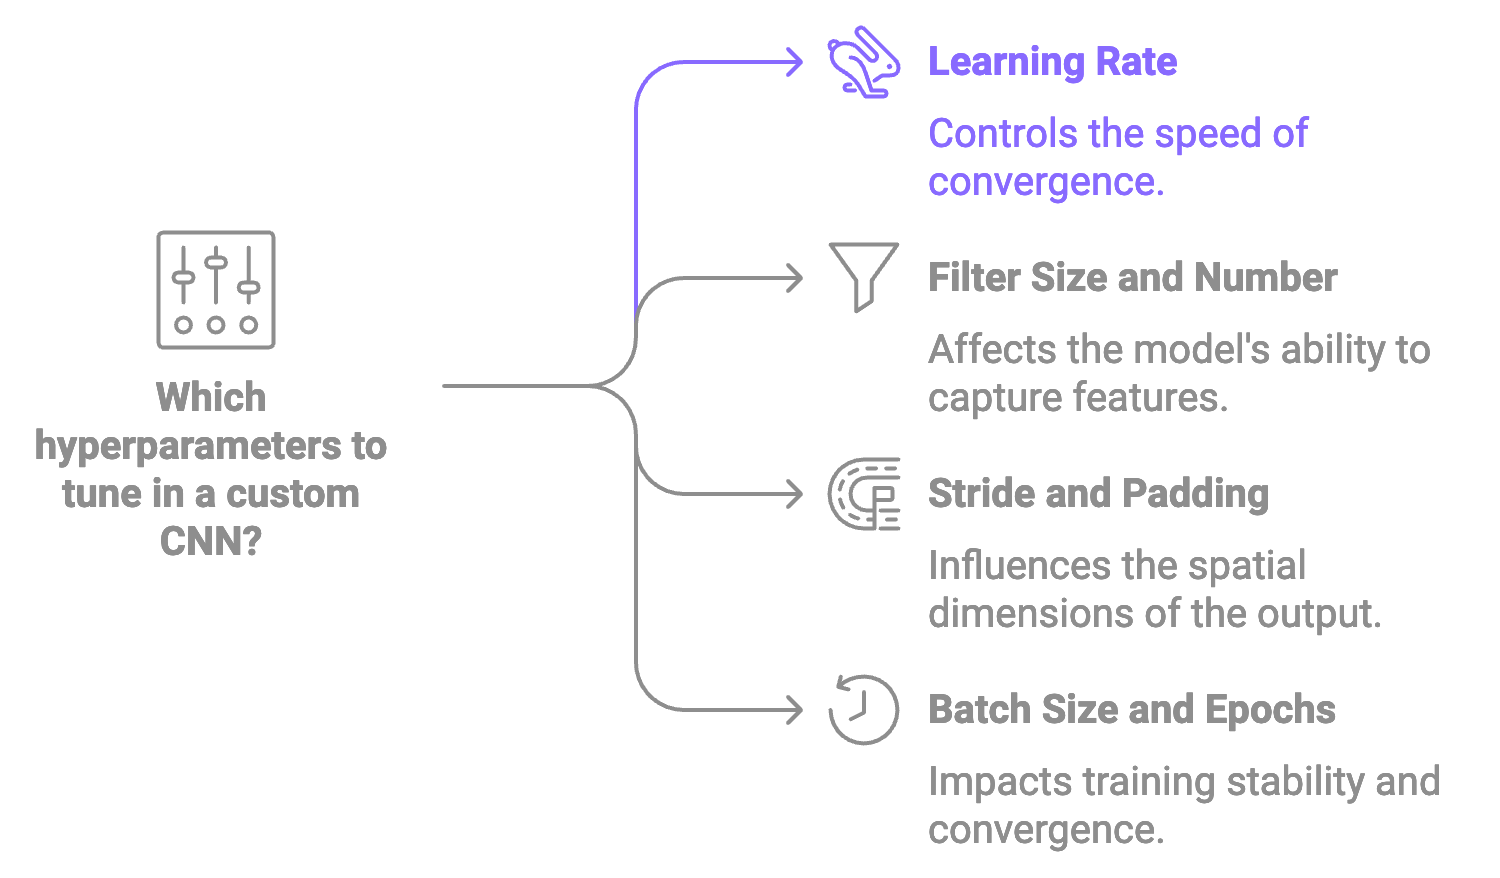
\includegraphics[width=\textwidth,height=0.35\textheight,keepaspectratio]{/Users/mac/Desktop/MST AISD/S3/Transfert Learning/TP/Image/napkin-selection (3).png}

\subsection{How is the model trained from scratch?}

Training a CNN from scratch involves several steps:

\begin{enumerate}
    \item \textbf{Initialization:} Initialize weights, commonly using Xavier or He initialization for stability.
    \item \textbf{Forward Pass:} Compute the output by passing input data through each layer.
    \item \textbf{Loss Calculation:} Calculate the loss, often cross-entropy for classification tasks:
    \[
    L = - \sum_{c=1}^C y_c \log(\hat{y}_c)
    \]
    where \( y_c \) is the true label and \( \hat{y}_c \) is the predicted probability for class \( c \).
    \item \textbf{Backward Pass (Backpropagation):} Compute the gradients of \( L \) with respect to each parameter using the chain rule.
    \item \textbf{Weight Update:} Adjust weights using an optimizer (e.g., SGD, Adam), iteratively reducing the loss.
    \item \textbf{Repeat:} Iterate through the training process for multiple epochs.
    \item \textit{Each step in the training process is designed to ensure that the model effectively learns the underlying patterns present in the data. By meticulously adjusting the model's parameters and continually refining its predictions through feedback, the network becomes increasingly adept at recognizing complex features and relationships within the dataset. This iterative learning process is crucial for improving the model's overall prediction accuracy, as it allows the network to adapt and generalize better to unseen data.}
\end{enumerate}




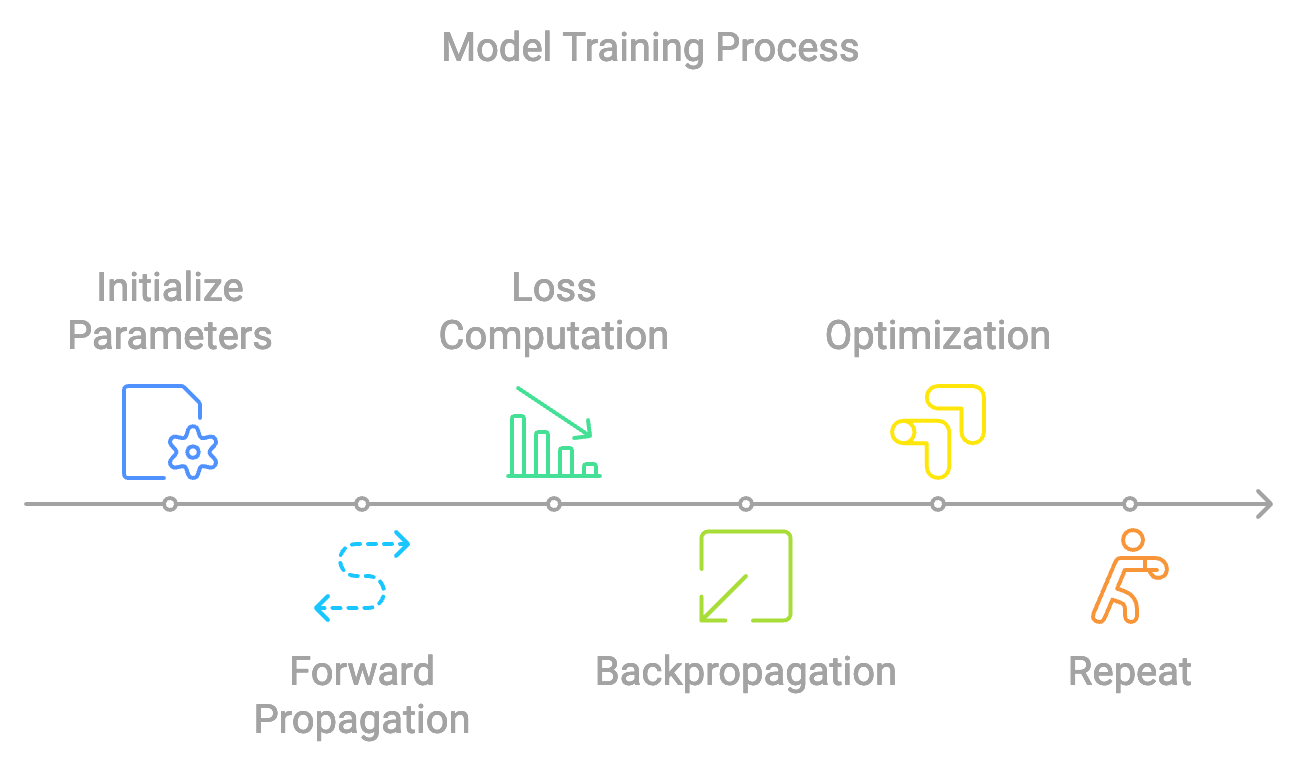
\includegraphics[width=\textwidth,height=0.35\textheight,keepaspectratio]{/Users/mac/Desktop/MST AISD/S3/Transfert Learning/TP/Image/napkin-selection4.png}

\subsection{How is a custom CNN evaluated?}

To evaluate a custom CNN, the following metrics and processes are typically used:

\begin{itemize}
    \item \textbf{Accuracy:} Measures the fraction of correct predictions.
    \item \textbf{Confusion Matrix:} Helps analyze classification performance by showing true positives, false positives, true negatives, and false negatives.
    \item \textbf{Precision, Recall, and F1 Score:} For imbalanced data, these metrics are crucial. For instance, precision is:
    \[
    \text{Precision} = \frac{\text{True Positives}}{\text{True Positives + False Positives}}
    \]
    and recall is:
    \[
    \text{Recall} = \frac{\text{True Positives}}{\text{True Positives + False Negatives}}
    \]
    F1 Score is the harmonic mean of precision and recall:
    \[
    \text{F1 Score} = 2 \cdot \frac{\text{Precision} \times \text{Recall}}{\text{Precision + Recall}}
    \]
    \item \textbf{Loss Curve:} By plotting the training and validation loss over epochs, we can visualize the model's learning process.
    \item \textbf{Test Set Evaluation:} The final test set provides an estimate of the model’s generalization to unseen data.
\end{itemize}

\begin{center}
    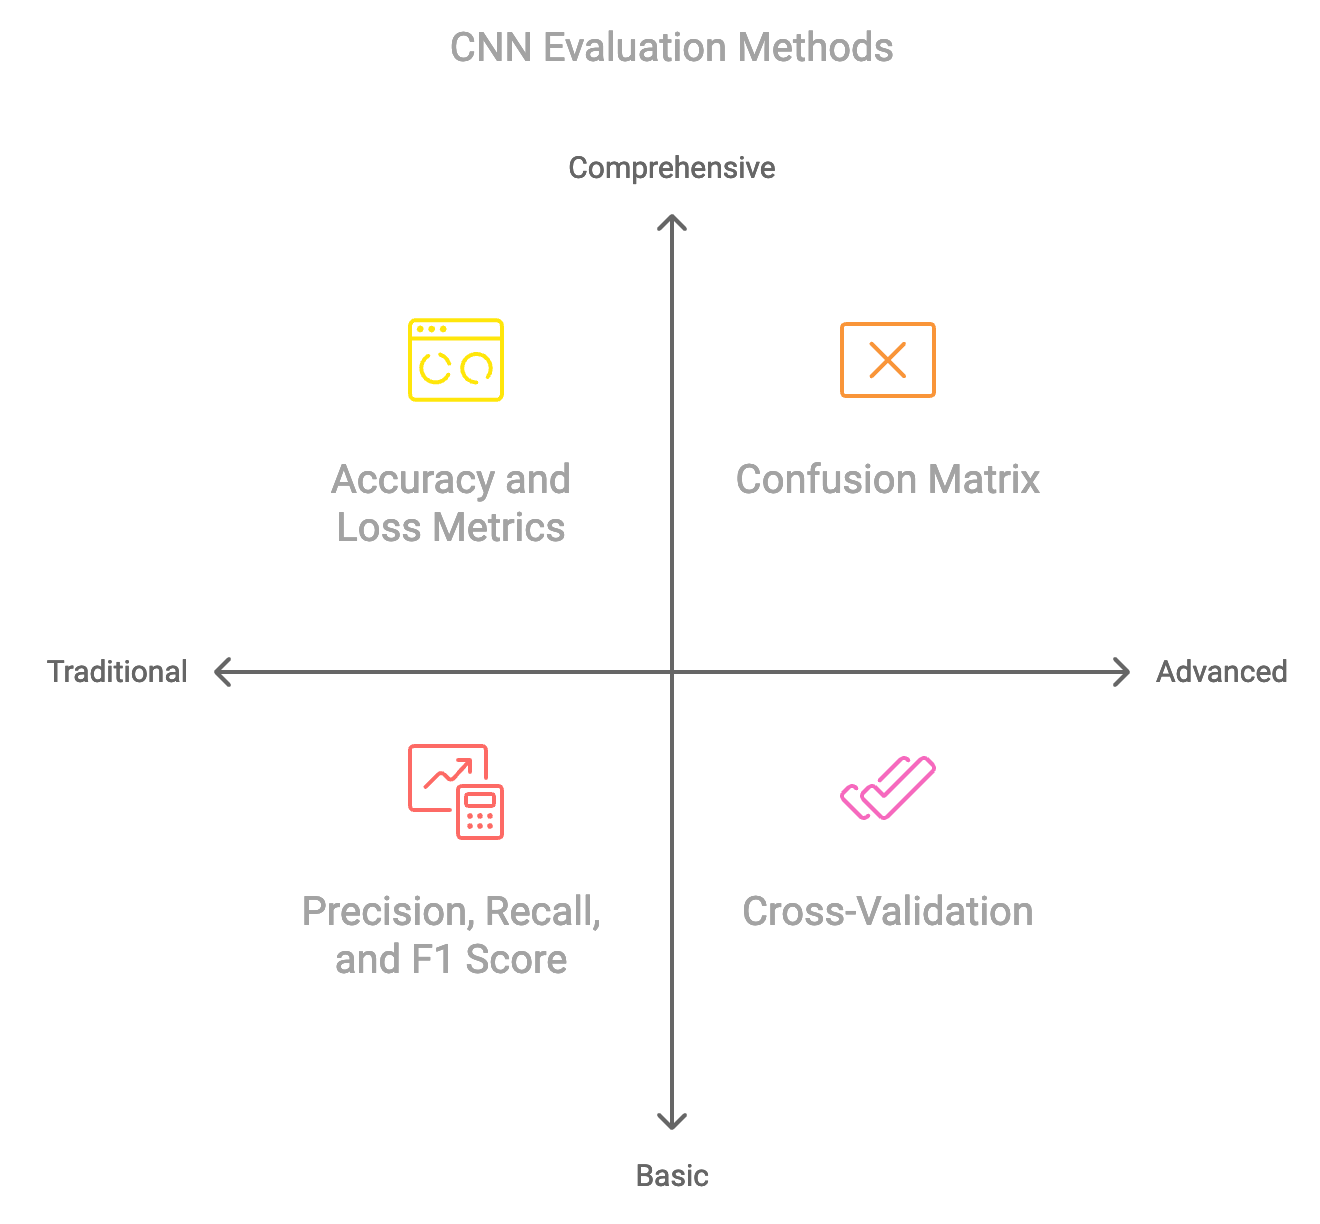
\includegraphics[width=\textwidth,height=0.35\textheight,keepaspectratio]{/Users/mac/Desktop/MST AISD/S3/Transfert Learning/TP/Image/napkin-selection6.png}
\end{center}
\newpage

\section{Exo 1: Image Prediction Using a Pre-Trained Model on ImageNet}

ImageNet is a database of over ten million labeled images, produced by the organization of the same name, aimed at research in computer vision.

\subsection{Question 01: How to load a pre-trained model on ImageNet with TensorFlow or PyTorch?}

\justify
To load a pre-trained model on ImageNet, you can use either TensorFlow or PyTorch, which offer predefined functions to access these models. 

\textbf{TensorFlow:} 

In TensorFlow, you can load a pre-trained model as follows:


This command loads the VGG16 model with weights pre-trained on ImageNet, allowing you to utilize the features extracted by this model in your own application.

\textbf{PyTorch:} 

In PyTorch, the process is similar:

\begin{lstlisting}

    import torchvision.modet as models
    model = models.resnet50(pretrained=True)
\end{lstlisting}

Here, `resnet50` is loaded with weights pre-trained on ImageNet, enabling you to benefit from the knowledge accumulated by this model.

\subsection{Question: Why is it necessary to resize images before using them with a pre-trained model?}

\justify
Resizing images is essential because pre-trained models on ImageNet were trained with specific image sizes (typically 224x224 pixels for many models). Reasons for resizing images include:

\begin{itemize}
    \item \textbf{Compatibility:} The input image dimensions must match those expected by the model. For example, if the model expects an image of \(224 \times 224\), providing an image of a different size will result in an error.
    \item \textbf{Normalization of Features:} By resizing all images to the same size, we ensure that the features extracted during training and prediction are consistent.
\end{itemize}

\subsection{Question: What is the importance of normalizing images before passing them into the pre-trained model?}

\justify
Normalizing images is crucial for several reasons:

\begin{itemize}
    \item \textbf{Value Scaling:} Pixel values of images should be normalized to avoid scale issues that can affect model performance. For example, if pixel values range from 0 to 255, we can normalize them by dividing by 255, bringing them into the range \([0, 1]\).
    \item \textbf{Distribution Centers:} Additionally, many models pre-trained on ImageNet use specific mean and standard deviation values for normalization. For example, for VGG16 and ResNet, normalization values often include:

    \[
    \text{mean} = [0.485, 0.456, 0.406], \quad \text{std} = [0.229, 0.224, 0.225]
    \]

    This centers the data around zero and ensures that pixel values are within an appropriate range for model training.
\end{itemize}

\subsection{Question: What steps should be followed to pass an image through a pre-trained model to obtain predictions?}

\justify
The typical steps to obtain predictions from an image using a pre-trained model include:

\begin{enumerate}
    \item \textbf{Load the image:} Use a library like PIL or OpenCV to read the image from disk.
    
    \item \textbf{Resize the image:} Adjust the image to the size required by the model, often \(224 \times 224\) pixels.
    
    \item \textbf{Normalize the image:} Apply normalization as described above. For example, to normalize using TensorFlow:
    
    \begin{lstlisting}
    from tensorflow.keras.preprocessing import image
    import numpy as np

    img = image.load_img('path_to_image.jpg', target_size=(224, 224))
    img_array = image.img_to_array(img) / 255.0  # Normalize to [0, 1]
    img_array = (img_array - np.array([0.485, 0.456, 0.406])) / np.array([0.229, 0.224, 0.225])  # Standard normalization
    img_array = np.expand_dims(img_array, axis=0)  # Add batch dimension
    \end{lstlisting}
    
    \item \textbf{Pass the image into the model:} Use the `predict` method to obtain predictions.
\end{enumerate}

\subsection{Question: How to interpret the prediction results of a pre-trained model on ImageNet?}

\justify
The prediction results of a pre-trained model on ImageNet are usually provided as probabilities for each class. To interpret these results, you can:

\begin{itemize}
    \item \textbf{Predicted class:} Identify the class with the highest probability using the `argmax` function. For instance, if the model returns a probability vector \([0.1, 0.3, 0.6]\), the predicted class is the one associated with \(0.6\).
    
    \item \textbf{Use a class mapping dictionary:} Map the class indices to class names to understand what each prediction means. The ImageNet classes are often available in a mapping file.
    
    \item \textbf{Visualize scores:} You can also display the probability scores for the top-N classes to get a better idea of other relevant classes. This can be done using a visualization library like Matplotlib.
\end{itemize}

\subsection{Question: Why use a pre-trained model on ImageNet for image prediction instead of building a model from scratch?}

\justify
Using a pre-trained model offers several advantages, including:

\begin{itemize}
    \item \textbf{Time-saving:} By using a pre-trained model, you save a significant amount of time that would have been needed to train a model from scratch, especially if you have a limited dataset.
    
    \item \textbf{Performance improvement:} Pre-trained models often have superior performance because they have been trained on a vast amount of varied data.
    
    \item \textbf{Learning rich features:} These models capture very general features that can be transferred to other tasks, which is crucial when working with smaller datasets.
\end{itemize}

\subsection{Question: What are the steps to fine-tune a pre-trained model on ImageNet for a new classification task? (TL)}

\justify
Fine-tuning a pre-trained model for a new classification task involves several steps:

\begin{enumerate}
    \item \textbf{Load the pre-trained model:} As mentioned, load a pre-trained model and remove the last layer to adapt the model for your new task.
    
    \item \textbf{Add new layers:} Add layers suitable for your task. For example, you might add a Dense layer with a number of neurons corresponding to the number of classes in your task.
    
    \item \textbf{Freeze some layers:} You can freeze certain layers to retain the learned weights. This is done by setting `layer.trainable = False` for the layers you wish to freeze.
    
    \item \textbf{Compile the model:} Use a new loss function, such as cross-entropy for classification tasks:

    \[
    L = - \sum_{c=1}^C y_c \log(\hat{y}_c)
    \]

    where \( y_c \) is the true label and \( \hat{y}_c \) is the predicted probability for class \( c \).
    
    \item \textbf{Train the model:} Train the model on your new dataset while monitoring performance on a validation set to avoid overfitting.
\end{enumerate}


\section{Image Classification with ResNet18}

In this subsection, we detail the process of classifying images using a pre-trained ResNet18 model. The model is employed to predict the classes of a set of images from a specified directory.

\subsection{Implementation Steps}

The following steps outline the implementation:

\begin{itemize}
    \item Load the pre-trained ResNet18 model.
    \item Prepare the images by applying necessary transformations.
    \item Implement a function to make predictions on the images.
    \item Loop through each image in the directory, process it, and display the predicted labels.
\end{itemize}

\subsection{Code Implementation}

Here is the code used for the image classification:

\begin{lstlisting}[language=Python, caption=Image Classification Code]
import torch
from torchvision import models, transforms
from PIL import Image
import matplotlib.pyplot as plt
import os
import json

# Load the Pre-trained Model
model = models.resnet18(pretrained=True)
model.eval()  # Set the model to evaluation mode

# Load the Label Mapping
with open("labels.json", "r") as f:
    labels = json.load(f)

# Define Preprocessing Transformations
preprocess = transforms.Compose([
    transforms.Resize(256),
    transforms.CenterCrop(224),
    transforms.ToTensor(),
    transforms.Normalize(mean=[0.485, 0.456, 0.406], std=[0.229, 0.224, 0.225]),
])

# Make Prediction Function
def predict(model, image_tensor):
    with torch.no_grad():
        outputs = model(image_tensor)
    _, predicted_class = outputs.max(1)
    return predicted_class.item()

# Loop Through Each Image in the Folder
image_folder_path = "path/to/images"
for image_name in os.listdir(image_folder_path):
    image_path = os.path.join(image_folder_path, image_name)
    
    if os.path.isfile(image_path) and image_name.lower().endswith(('.png', '.jpg', '.jpeg')):
        img = Image.open(image_path).convert("RGB")
        img_tensor = preprocess(img).unsqueeze(0)
        predicted_index = predict(model, img_tensor)
        predicted_label = labels[predicted_index] if predicted_index < len(labels) else "Unknown"
        
        # Display the image and prediction
        plt.imshow(img)
        plt.title(f"Predicted Class: {predicted_label}")
        plt.axis('off')
        plt.show()
\end{lstlisting}
\newpage
\subsection{Output Results}

The following images show the results of the predictions made by the model on the input images:
\begin{center}
    \begin{minipage}{0.3\textwidth}
        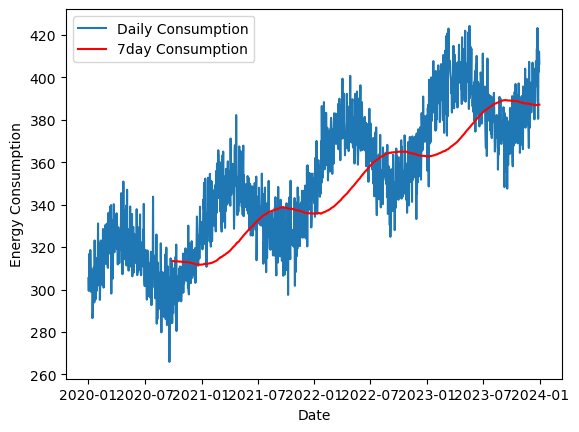
\includegraphics[width=\textwidth]{/Users/mac/Desktop/MST AISD/S3/Transfert Learning/TP/Image/output.png}
        \captionof{figure}{Predicted Class: Chameleon}
    \end{minipage}
    \hspace{1cm} % Adjust space between images
    \begin{minipage}{0.3\textwidth}
        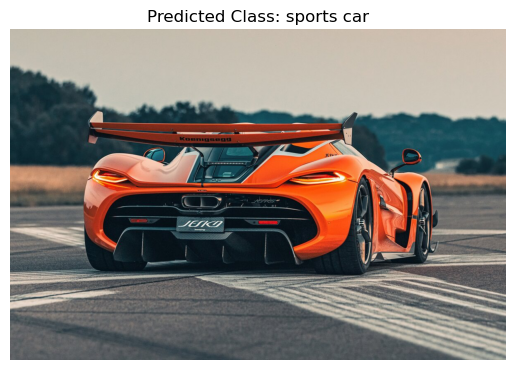
\includegraphics[width=\textwidth]{/Users/mac/Desktop/MST AISD/S3/Transfert Learning/TP/Image/output2.png}
        \captionof{figure}{Predicted Class: Sport Car}
    \end{minipage}
    \hspace{1cm} % Adjust space between images
    \begin{minipage}{0.3\textwidth}
        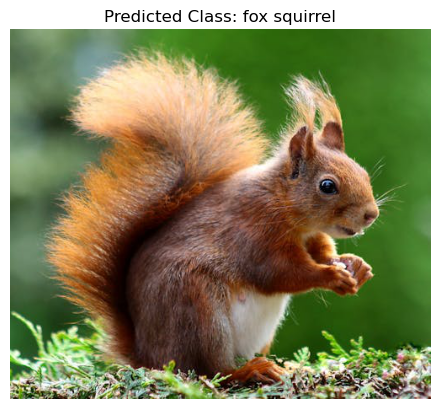
\includegraphics[width=\textwidth]{/Users/mac/Desktop/MST AISD/S3/Transfert Learning/TP/Image/output1.png}
        \captionof{figure}{Predicted Class: Fox Squirrel}
    \end{minipage}
\end{center}
\newpage

\section{Exercice 3 : CNN 1D,2D, and 3D}

\subsection{Main Difference Between CNN 1D, 2D, and 3D}
\begin{center}
    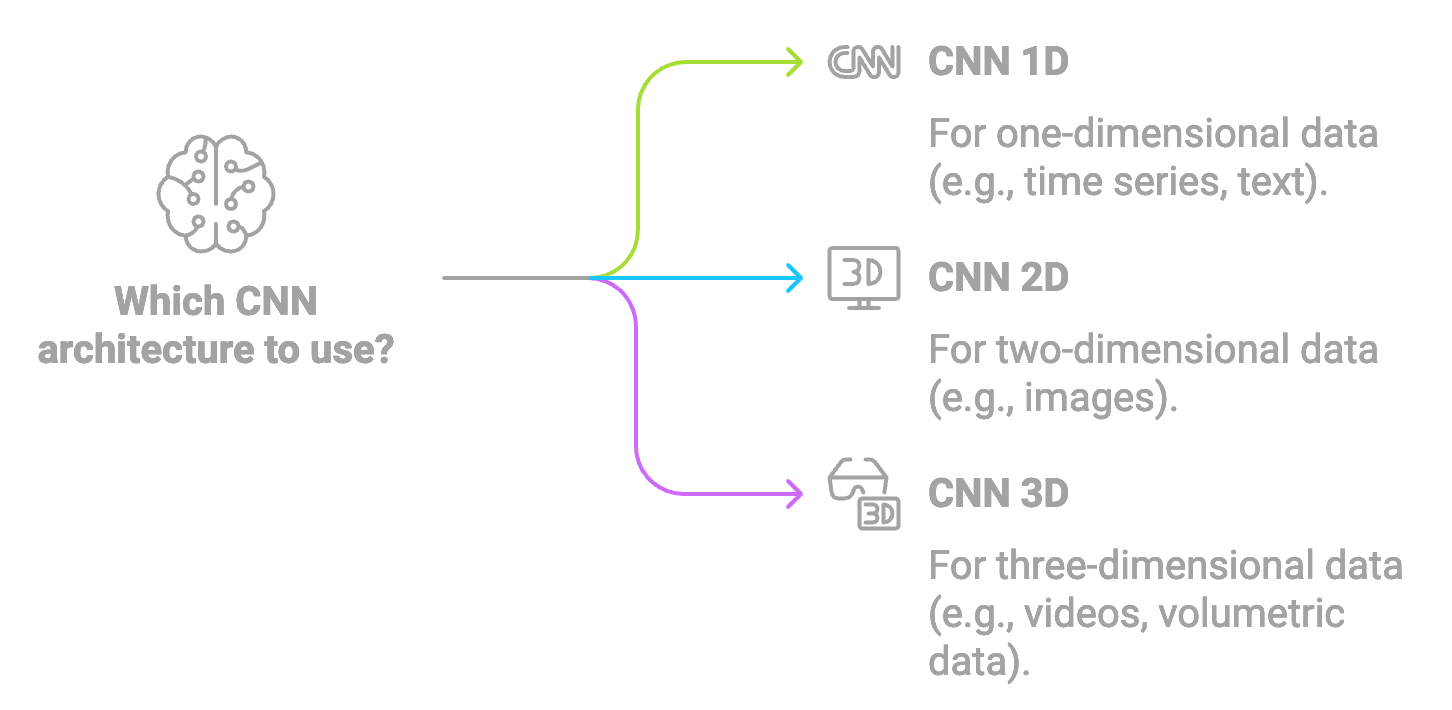
\includegraphics[width=0.7\textwidth]{/Users/mac/Desktop/MST AISD/S3/Transfert Learning/TP/Image/napkin-selection 6.png}    
\end{center}

\paragraph{1D Convolutional Neural Networks:} 
These networks are specifically designed for one-dimensional data, such as time series or text sequences. In CNN 1D, convolution operations are applied along a single axis, enabling the model to capture temporal or sequential patterns effectively.

\paragraph{2D Convolutional Neural Networks:} 
CNNs of this type are utilized for processing images or data that are structured in two dimensions. In 2D CNNs, convolution operations are performed over two axes—height and width—allowing the model to extract spatial features and patterns within the images.

\paragraph{3D Convolutional Neural Networks:} 
These networks are employed for volumetric data or video sequences, where convolution operations are applied across three axes—height, width, and depth. CNN 3D is adept at capturing spatial and temporal information, making it ideal for tasks such as action recognition in videos or processing 3D medical imaging data.

\subsection{How a Convolution Layer Works in a CNN 1D}
In a CNN 1D, a convolution layer applies a filter (or kernel) that slides along the one-dimensional input. Each position of the filter produces a value by multiplying the filter elements with the corresponding elements in the input region. The result is a feature map that captures the patterns present in the input sequence. The output size is determined by the filter size, stride, and padding.

\subsection{When and Why to Use a CNN 3D}
A CNN 3D is used when it is necessary to capture information in volumetric data, such as videos, medical images (like MRIs), or 3D simulations. It is particularly useful when spatial and temporal relationships need to be considered simultaneously, for example, for action classification in video sequences or volume analysis in medical data.

\subsection{Examples of 3D Data}
An example of 3D data is a video, which can be represented as a sequence of successive 2D images with a temporal dimension. Another example is a volume of medical images, such as an MRI scan, which contains multiple slices (2D) of an organ at different depths.

\subsection{Differences in Pooling Layers Between CNN 1D, 2D, and 3D}
\begin{itemize}
    \item \textbf{1D Pooling:} Reduces the size of one-dimensional feature maps by applying a downsampling operation (max or average) over consecutive segments of the single dimension.
    \item \textbf{2D Pooling:} Reduces the size of 2D feature maps by applying downsampling over rectangular regions (height and width) within each image.
    \item \textbf{3D Pooling:} Reduces the size of 3D feature maps by applying downsampling over cubic blocks of data (height, width, and depth), which helps preserve spatial and temporal information.
\end{itemize}

\subsection{Specific Challenges of CNN 3D Compared to CNN 2D}
The challenges of CNN 3D include:
\begin{itemize}
    \item \textbf{Computational Complexity:} CNN 3D requires more computational resources and memory due to the larger volume of data, making training time-consuming and costly.
    \item \textbf{Overfitting:} With more parameters to learn, there is an increased risk of overfitting, especially if the datasets are limited.
    \item \textbf{Data Preprocessing:} Managing volumetric data may require more sophisticated preprocessing techniques to ensure data quality and consistency in learning.
\end{itemize}

\newpage
\section{Implementation of CNN 1D on Energy Consumption Data}

In this section, we implement a 1D Convolutional Neural Network (CNN) to analyze energy consumption data. The data is read using the following code:

\begin{lstlisting}[language=Python,]
df = pd.read_csv('../datasets/d5.csv')
\end{lstlisting}

All interpretations of the data were made in the previous report where we worked with Long Short-Term Memory (LSTM) networks. To prepare our data for the CNN, we start by defining a Z-score function to standardize our input data:

\begin{lstlisting}[language=Python,]
def zscore(s, window, thresh=1, return_all=False):
    roll = s.rolling(window=window, min_periods=1, center=True)
    avg = roll.mean()
    std = roll.std(ddof=0)
    z = s.sub(avg).div(std)
    m = z.between(-thresh, thresh)
    
    if return_all:
        return z, avg, std, m
    return s.where(m, avg)
\end{lstlisting}

The Z-score normalization is defined mathematically as:

\begin{center}
\[
Z = \frac{X - \mu}{\sigma}
\]
\end{center}

where \(Z\) is the Z-score, \(X\) is the original value, \(\mu\) is the mean of the values, and \(\sigma\) is the standard deviation. This transformation ensures that the data has a mean of 0 and a standard deviation of 1.

Next, we transformed our data into sequences with a window size of 15 days, which allows the model to capture temporal patterns in energy consumption. After this, we standardized our data using MinMaxScaler, which scales the data to a fixed range, typically [0, 1].

We then converted our feature and target variables (\(X\) and \(Y\)) into tensors for use in PyTorch.

The architecture of our CNN model is defined in the following class:

\begin{minipage}{\textwidth}
    \begin{lstlisting}[language=Python,]
    class EnergyCNN1D(nn.Module):
        def __init__(self, input_size=15, output_size=1, num_filters=64, kernel_size=1, num_layers=1):
            super(EnergyCNN1D, self).__init__()
            self.conv_layers = nn.ModuleList()
            for i in range(num_layers):
                in_channels = input_size if i == 0 else num_filters
                self.conv_layers.append(nn.Conv1d(in_channels, num_filters, kernel_size=kernel_size))
                self.conv_layers.append(nn.ReLU())
            self.fc = nn.Linear(num_filters, output_size)
    
        def forward(self, x):
            for layer in self.conv_layers:
                x = layer(x)
            
            x = x.view(x.size(0), -1)  # Flattening the output
            out = self.fc(x)
            return out
    \end{lstlisting}
    \end{minipage}

The key components of the CNN are:

1. **Convolutional Layer**: This layer applies a convolution operation to the input, which helps to learn spatial hierarchies in the data. The mathematical operation for a 1D convolution is given by:

\begin{center}
\[
Y[i] = \sum_{j=0}^{k-1} X[i+j] \cdot W[j] + b
\]
\end{center}

where \(Y[i]\) is the output, \(X\) is the input, \(W\) is the filter (kernel), \(b\) is the bias, and \(k\) is the kernel size.

2. **Activation Function**: We used the ReLU (Rectified Linear Unit) activation function, which is defined as:

\begin{center}
\[
\text{ReLU}(x) = \max(0, x)
\]
\end{center}

This function introduces non-linearity to the model, enabling it to learn complex patterns.

3. **Fully Connected Layer**: After the convolutional layers, a fully connected layer is used to produce the final output. It connects every neuron in the last convolutional layer to the output neurons.

We instantiated the model with the following parameters:

\begin{lstlisting}[language=Python,]
input_size = 1
hidden_layer_size = 50
output_size = 1
num_layers = 3
model = EnergyCNN1D(input_size=15, output_size=1, num_filters=64, kernel_size=1, num_layers=2)
\end{lstlisting}

To examine the model's output shape, we utilized:

\begin{lstlisting}[language=Python,]
outputs = model(X_train)
print(outputs.shape)
\end{lstlisting}

We defined our loss function and optimizer as follows:

\begin{lstlisting}[language=Python,]
criterion = nn.MSELoss() 
optimizer = torch.optim.Adam(model.parameters(), lr=0.001)
\end{lstlisting}

The Mean Squared Error (MSE) loss is calculated using:

\begin{center}
\[
\text{MSE} = \frac{1}{n} \sum_{i=1}^{n} (y_i - \hat{y}_i)^2
\]
\end{center}

where \(y_i\) is the actual value, \(\hat{y}_i\) is the predicted value, and \(n\) is the number of observations. This loss function is particularly useful for regression tasks as it measures the average squared difference between the predicted and actual values.

The training process was conducted over 100 epochs, recording training and validation losses:

\begin{lstlisting}[language=Python,]
num_epochs = 100
train_losses = []
val_losses = []

for epoch in range(num_epochs):
    model.train()
    optimizer.zero_grad()
    outputs = model(X_train)
    train_loss = criterion(outputs, y_train.view(-1, 1))
    train_loss.backward()
    optimizer.step()
    train_losses.append(train_loss.item())
    
    model.eval()
    with torch.no_grad():
        val_outputs = model(X_test)
        val_loss = criterion(val_outputs, y_test.view(-1, 1))
        val_losses.append(val_loss.item())
        
    if (epoch + 1) % 10 == 0:
        print(f'Epoch [{epoch + 1}/{num_epochs}], Train Loss: {train_loss.item():.4f}, Validation Loss: {val_loss.item():.4f}')
\end{lstlisting}

After training, we calculated metrics on the validation set:

\begin{lstlisting}[language=Python,]
with torch.no_grad():
    final_outputs = model(X_test)
    
    y_test_np = y_test.view(-1, 1).cpu().numpy()
    final_outputs_np = final_outputs.cpu().numpy()
    
    mse, rmse, r2 = compute_metrics(y_test_np, final_outputs_np)
    
    print(f'Validation MSE: {mse:.4f}')
    print(f'Validation RMSE: {rmse:.4f}')
    print(f'Validation R square: {r2:.4f}')
\end{lstlisting}

The results obtained after training were as follows:

\begin{lstlisting}[language=Python,]
Epoch [10/100], Train Loss: 0.0015, Validation Loss: 0.0018
Epoch [20/100], Train Loss: 0.0015, Validation Loss: 0.0018
Epoch [30/100], Train Loss: 0.0015, Validation Loss: 0.0018
Epoch [40/100], Train Loss: 0.0015, Validation Loss: 0.0018
Epoch [50/100], Train Loss: 0.0014, Validation Loss: 0.0018
Epoch [60/100], Train Loss: 0.0014, Validation Loss: 0.0018
Epoch [70/100], Train Loss: 0.0014, Validation Loss: 0.0018
Epoch [80/100], Train Loss: 0.0014, Validation Loss: 0.0018
Epoch [90/100], Train Loss: 0.0014, Validation Loss: 0.0018
Epoch [100/100], Train Loss: 0.0014, Validation Loss: 0.0018
Validation MSE: 0.0018
Validation RMSE: 0.0426
Validation R square: 0.9682
\end{lstlisting}
\newpage
\subsubsection{Interpretation of Results}
The training and validation losses show a decreasing trend over the epochs, indicating that the model is learning effectively. 

- \textbf{Training Loss:} The training loss decreased from \(0.0015\) to \(0.0014\), demonstrating the model's improvement in fitting the training data.
- \textbf{Validation Loss:} The validation loss remained relatively stable at around \(0.0018\) throughout the training process. This stability suggests that the model is generalizing well to unseen data, with no significant \textbf{overfitting} occurring.

The validation metrics further indicate strong performance:
- \textbf{Mean Squared Error (MSE):} The MSE of \(0.0018\) indicates low average squared differences between predicted and actual values.
- \textbf{Root Mean Squared Error (RMSE):} An RMSE of \(0.0426\) suggests that the model's predictions deviate, on average, by approximately \(0.0426\) from the actual values, which is acceptable in the context of \textbf{energy consumption data}.
- \textbf{R² Score:} An \(R^2\) value of \(0.9682\) signifies that about \(96.82\%\) of the variance in the validation dataset can be explained by the model, indicating a good fit.

Overall, the results suggest that the \textbf{EnergyCNN1D} model is effective in predicting energy consumption based on the given dataset.

\begin{center}
    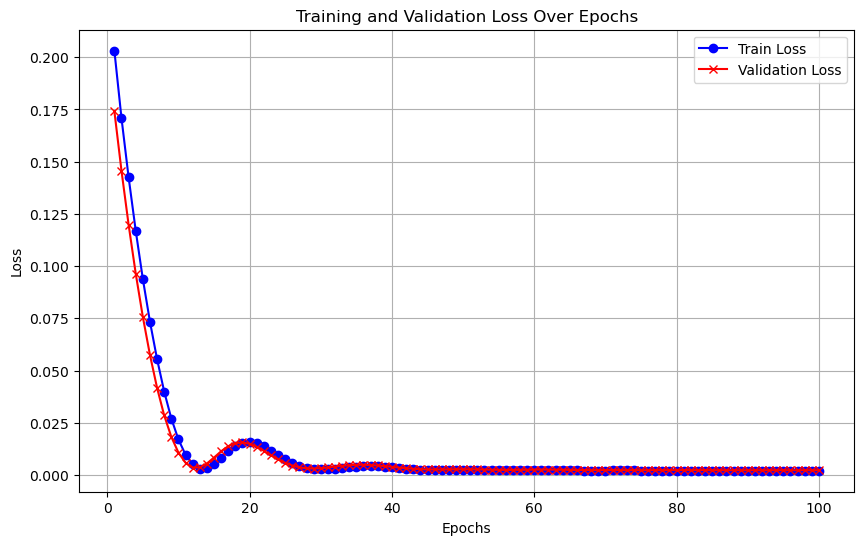
\includegraphics[width=\textwidth,height=0.25\textheight,keepaspectratio]{/Users/mac/Desktop/MST AISD/S3/Transfert Learning/TP/Image/last.png}
\end{center}

\end{document}